% $Id$

\documentclass[a4paper,10pt]{article}
\usepackage[a4paper,inner=1in,outer=1in,top=1in,bottom=1.5in]{geometry}
\usepackage{setspace}
%\usepackage[pdftex]{color,graphicx}
\usepackage[dvips]{color,graphicx}
\usepackage{verbatim}
\usepackage{./sty/algorithm2e}
\usepackage{epsfig}
\usepackage{subfigure}
\usepackage{listings}
\usepackage{url}
\usepackage{fancyhdr}
\usepackage{multirow}
\usepackage{amsmath}
\usepackage{amsfonts}

\bibliographystyle{abbrv}
\DeclareGraphicsRule{*}{eps}{*}{}

\title{Congestion Control for Real-time Mulimedia Application}
\author{Soo-Hyun Choi}

%%% CHECK IF PDFLATEX OR LATEX
%\ifx\pdftexversion\undefined
%  \usepackage[dvips]{color,graphicx}
%\else  
%  \pdfpagewidth=\paperwidth
%  \pdfpageheight=\paperheight
%  \usepackage[pdftex]{color,graphicx}
%  \usepackage[pdftex, colorlinks, %
%	pdfauthor = {Soo-Hyun Choi}, %
%	pdftitle = {Design and Analysis for TCP-Friendly Window-based 
%				Congestion Control},%
%	citecolor = black, %
%	filecolor = black, %
%	linkcolor = black, %
%	urlcolor = black]{hyperref}
%\fi

\begin{document}

%%%%%%%%%%%%%%%%% TITLE PAGE
\begin{titlepage}
\begin{center}
%\includegraphics{logo}
\vspace*{\stretch{1}}
{\LARGE \textsf{\textbf{Congestion Control for Real-time Multemida Application 
\\}}}
\vspace{.5cm}
{\large \textsf{\textbf{Project Plan}}\\}
\vspace{1cm}
{\large \textsf{Soo-Hyun Choi\\}}
{\small \textsf{s.choi@cs.ucl.ac.uk}\\}
{\small \textsf{+44 (0)20 7679 0352}\\}
{\small \url{http://www.cs.ucl.ac.uk/staff/s.choi}\\}
\vspace{2.5cm}
{\large \textsf{Supervised by \\
Piers O'Hanlon and Colin Perkins \\}}
\vspace{2.0cm}
{\normalsize \textbf{Keywords}\\Internet congestion control, Real-time
multimedia application}
\end{center}
\vspace*{\stretch{1}}

\vspace{2cm}
\vspace*{\stretch{1}}
\begin{small}
\begin{center}

\includegraphics[scale=.15]{./img/ucl_logo} \\
\vspace{1cm}
A document submitted in partial fulfillment \\
of the requirement for \\
\textsf{\textbf{Google Summer of Code (GSoC) 2008}} \\
\vspace{1cm}
\textsf{\today}
\end{center}
\end{small}
\vspace*{\stretch{1}}

\end{titlepage}

%% Abstract
\thispagestyle{empty}
\vspace*{\stretch{.5}}
\begin{center}
    \begin{abstract}
    % $Id$

\vspace{.5cm} 

\begin{center} 

This article describes the initial design plan for \textsf{Google Summer of Code
2008} under
\textsf{AVATS}\footnote{\textsf{http://www.cs.ucl.ac.uk/research/avats/}}.

\end{center}

    \end{abstract}
\end{center}
\vspace*{\stretch{1}}
\clearpage
\newpage


%%%%%%%%%%%%% DEDICATION
%\thispagestyle{empty}
%\vspace*{\stretch{1}}
%\begin{center}
%{\large\em To my family \ldots}
%\end{center}
%\vspace*{\stretch{1}}
%\clearpage

%%%%%%%%%%%%% TOC / HEADER DEF
\pagestyle{fancy}
\addtolength{\headheight}{\baselineskip}
\newcommand{\chaptermark}[1]{%
\markboth{#1}%
{}}
\lhead{}
\chead{}

\rhead{\nouppercase{{\sl \leftmark}} \hspace{0.5cm} \makebox[1cm][r]{%
\thepage}}

\cfoot{}

\fancypagestyle{plain}{%
\fancyhf{}
\renewcommand{\headrulewidth}{0pt}
\fancyfoot[R]{\thepage}
}

\tableofcontents
\newpage
%\listoffigures
%\newpage 
%\listofalgorithms
%\listoftables

%%%%%%%%%%%%%% START
\section{\label{sec:intro}Introduction}
% $Id$

\emph{vic/rat}~\cite{MEDIATOOLS} is a media tool that can have interactive
real-time audio/video conference. These tools have been used in many relevant
research projects such as AccessGrid~\cite{ACCESSGRID}, AVATS~\cite{AVATS} and
UltraGrid~\cite{UltraGrid}. Currently, \emph{vic/rat} is supported by AVATS
project~\cite{AVATS}. \emph{vic} supports many video codecs since its initial
development and implements RTP/RTCP protocol~\cite{RTP} over UDP to increase
interoperability. In this year's GSoC project, we would like to implement
congestion control protocols (TFRC and TFWC) over \emph{vic}. 

\subsection{\label{ssec:project_overview}Overview}

Recently, TCP-Friendly Rate-based congestion control protocol, ala
TFRC~\cite{FHPW00}, has been proposed and it is now being standardized by IETF
under DCCP CCID3~\cite{CCID3}. The main advantages of using this protocol are 1)
it can generate smooth and predictable sending rate 2) it can help timely packet
delivery. However, TFRC might be too much aggressive against TCP sources in some
environment or it might be too much unresponsive to generate a useful sending
rate in some other network environment. To solve this issue, a window-based
version of TFRC has been proposed: TCP-Friendly Window-based Congestion Control
(TFWC)~\cite{SH06} and~\cite{CH07}.

\subsection{\label{ssec:motivation}Motivation}

The motivation of implementing congestion control mechanisms over such a
multimedia application (e.g.\emph{vic} or \emph{rat}) is that we can have a good
controllability at the sending/receiving buffer to make the overall end-to-end
packet delay be within a certain level of timing requirements. Considering the
fact that the delay (and delay jitter) is one of the critical parameters that a
user might greatly care, the controlled delay using congestion control mechanism
could bring a significant advantage to those applications.

\subsection{\label{ssec:aims}Aims and Objectives}

The main project aim in this GSoC 2008 is to implement TFR(W)C over \emph{vic}, and it
can be (roughly) sub-categorized with short descriptions as belows:

\begin{enumerate} %% start enumerating

\item \textbf{TFR(W)C}

\begin{itemize}
\item \textsf{sender/receiver} -- protocol implementation
\item \textsf{CC handler} -- generic congestion control function handler
\item \textsf{RTP for TFR(W)C} -- RTP interface with TFR(W)C
\item \textsf{RTP} -- RTP extension
\end{itemize}

\item \textbf{Buffers}
\begin{itemize}
\item \textsf{send buffer (sbuf)} --  maintain send buffer context (e.g., frame
length, number of frames, send time to transmit a frame, and etc.)
\item \textsf{receive buffer (rbuf)} -- de-queue received frames
\end{itemize}

\item \textbf{Codecs}
\begin{itemize}
\item \textsf{video codecs} -- ability to change encoding rates based on the
feedback information from CC mechanisms
\end{itemize}

\item \textbf{Test Modules}
\begin{itemize}
\item \textsf{packet gen} -- dummy packet generator to test TFR(W) protocol
implementation at the initial development stage
\item \textsf{traffic gen} -- traffic generator to evaluate \emph{vic} with CC
mechanisms
\end{itemize}

\end{enumerate} %% end enumerating

Roughly speaking, there are 5 components to be developed in this project: TFRC,
TFWC, Buffers, Codecs, and Test Modules. We discuss some design/development
issues in the following subsections.

\subsubsection{\label{sssec:aim:cc}TFR(W)C Implementation}

We hope that we could nicely re-use TFR(W)C implementation from
UltraGrid~\cite{UltraGrid} and ns-2 version of TFWC~\cite{SH06}, respectively.
Although the base architecture is different from what those codes, we still
think that we can refer much of their codes. However, we still do not have a
concrete idea which part can be re-used or which part cannot.

\subsubsection{\label{sssec:aim:buffers}Buffers}

The packet buffer in the current \emph{vic} implementation~\cite{AVATS} seems to be
primitive stage - i.e., it does not have fine control of the packet buffer
queue.  As we expect CC mechanisms can provide network information (and should
be able to maintain various state variables) to the upper layer (e.g., video
codecs), the extended version of the current packet buffer is necessary. But, it
is currently not decided what kind of context should be maintained in each
buffers (send buffer and receive buffer).

\subsubsection{\label{sssec:aim:codecs}Codecs}

Firstly, we need to find appropriate video codecs that can be used with CC
mechanisms. The ideal codec can be the one which can adapts framing rate on the
fly without re-initializing it. If this is not supported in any of the current
codecs, we could modify them in a number of different ways to reflect the
feedback information from CC mechanisms. Or, we could manipulate Q-factor in
each codec on the fly based on the feedback information. Again, all of these
decision are not made yet.

\subsubsection{\label{sssec:aim:test}Test Modules}

After implementing TFR(W)C protocols, we would be faced with the point where we
need to test our implementation. There are two things involved in this
component: packet generator and traffic generator. The encoders in the current
\emph{vic} can only take YUV, JPEG, DCT, H261, and CellB Frames\footnote{See
\texttt{module.h} under \emph{vic} home directory.}. Therefore, in order to test our CC
implementation, we need to generate packets in one of those video format. Or, we
could simply use pre-recorded video sequences to transmit for the test purpose.
Next, it's necessary to generate traffic in a real network (or a dummy network)
for that purpose.

\subsection{\label{ssec:structure}Structure of the Report}

This report is organized as follows. In order to get an idea on integrating the
congestion control modules in \emph{vic}, we describe the basic working
mechanisms of UltraGrid~\cite{UltraGrid} in Section~\ref{sec:ultragrid}.
Section~\ref{sec:overview} describes the high-level overview of \emph{vic}
architecture and also gives an examples how the still grabber generates packets
over the network. Section~\ref{sec:cc-api} describes our proposed congestion
control APIs and how it could be integrated in \emph{vic}.
Section~\ref{sec:summary} summarized the project milestones and the expected
outcomes.

\newpage



\section{\label{sec:overview}Project Overview}
% $Id$

\subsection{\label{ssec:high-arch}High-level, proposed \emph{vic} Architecture}

We have drawn a high-level overview of the proposed \emph{vic} architecture
(sender only) that has congestion control modules as in
Figure~\ref{fig:high-vic-arch}.  This figure represents a high-level overview of
\emph{vic} so that we could see the major components of the system, and how they
are interacting with each other. 

\vspace{1cm}

\begin{figure}[!h]
\begin{center}
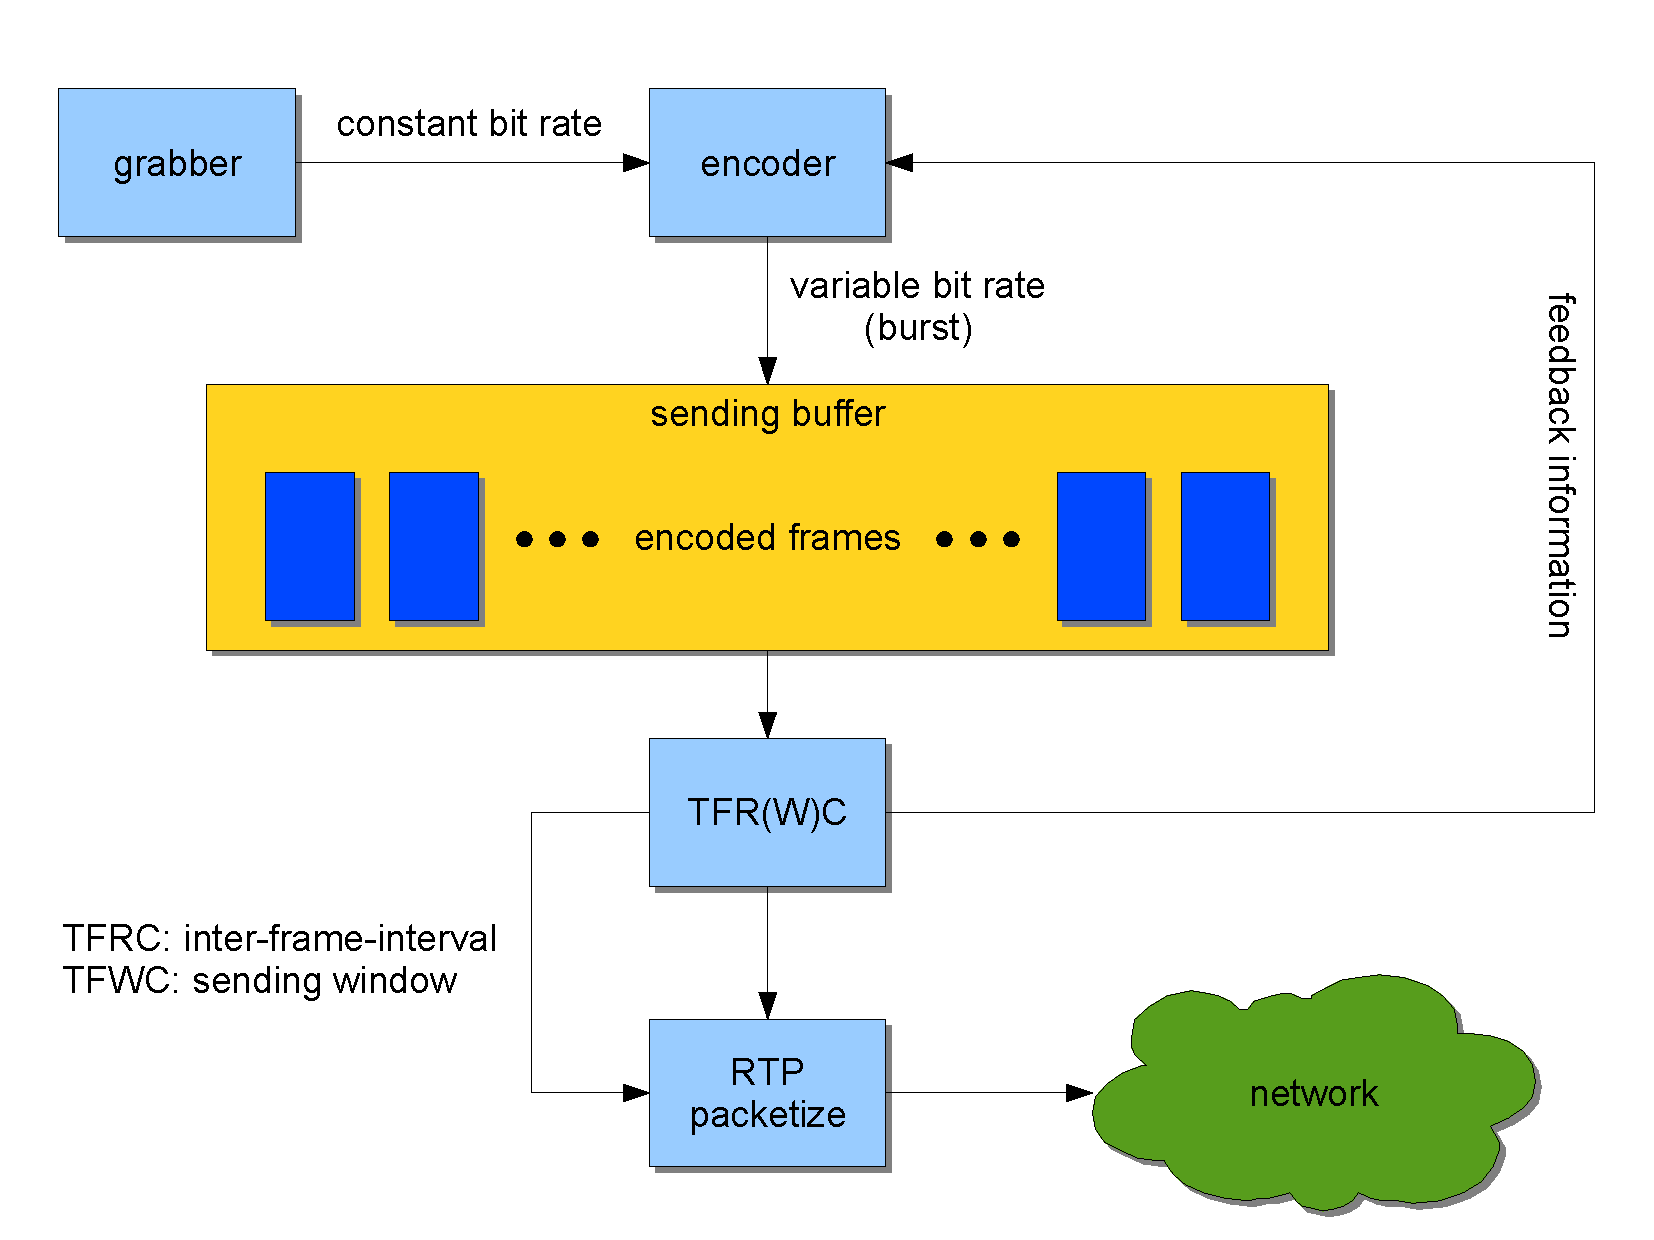
\includegraphics[scale=.5]{./img/high-vic-arch}
\caption{\label{fig:high-vic-arch}High-level, proposed \emph{vic} Architecture 
with CC Mechanisms}
\end{center}
\end{figure}

Unlike to the sender, we envisage the architecture of the receiver is relatively
simple. For example, upon a packet reception, it will be inserted to a receive
buffer, subsequently decoded (and some color conversion if necessary), and
finally displayed in a output device. Depending upon a codec, the rendered
frames may not be discarded immediately, but will be kept for some times before
they get purged.

\subsection{\label{ssec:vic-overview}\emph{vic} Overview by Example}

In this subsection, we describe how \emph{vic} works. To do so, we take the
still grabber (\texttt{grabber-still.cpp}) as an example and describe how
packets are transmitted.  The purpose of this analysis is to figure out how
\emph{vic} works and, from that, we would like to know how to design the
congestion control APIs. The still grabber can be used when we want to feed
pre-recored video sequences to the \emph{vic} system\footnote{One should start
\emph{vic} using the following command: \texttt{./vic -XstillGrabber \emph{(IP
address)}/\emph{(port number)}}.}. Currently, the still grabber in \emph{vic}
can take a JPG image file (4:2:2) and a CIF formatted video file.
Figure~\ref{fig:still-grabber} shows a class-diagram like figure that how the
still grabber generates packets. \\

\begin{figure}[!h] 
\begin{center}
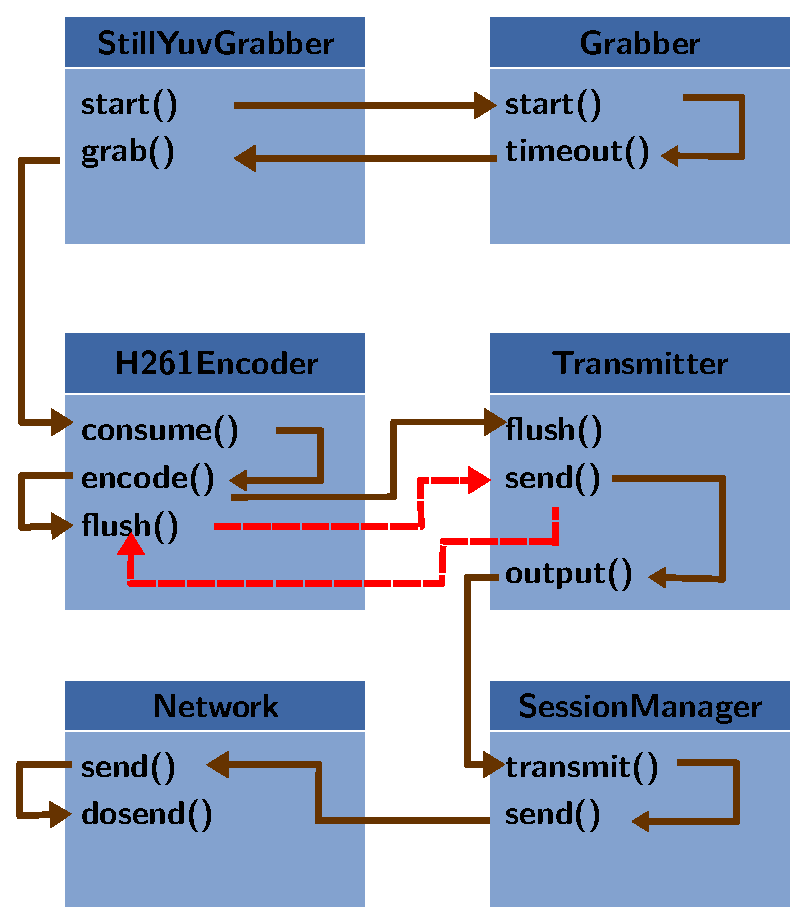
\includegraphics[scale=.5]{./img/still-grabber}
\caption{\label{fig:still-grabber}Still Grabber Information Flow}
\end{center} 
\end{figure}

Once the still device loads a file (either a JPG or a CIF file) into the memory,
it invokes \texttt{StillGrabber} or \texttt{StillYuvGrabber} depending upon a
file type. Assuming \texttt{StillYuvGrabber} is called, it sets the frame size
by calling \texttt{setsize()} method, and calls
\texttt{StillYuvGrabber::start()} which again calls \texttt{Grabber::start()}.
\texttt{Grabber::start()} basically sets the frame clock and timer using
\texttt{timeout()} method.  Then, \texttt{StillYuvGrabber::grab()} starts
grabbing video frames from the memory and passes to the encoder
(\texttt{encoder-h261.cpp}): in this case, \texttt{H261PixelEncoder::consume()}
will be called. After that, it starts encoding macro-blocks given a set of YUV
inputs and send the encoded frames to the transmit module
(\texttt{SessionManager::transmit()}). The encoder provides the encoded frames
to the transmit module as long as they are available: see the dashed line in
Figure~\ref{fig:still-grabber}.  \texttt{SessionManager::transmit()} then
packetizes the frames and sends it to the network. \\

This is an example of how \emph{vic} takes input from a file, encodes the
frames, packetizes them, and sends them to the network. The core part of the
congestion control module could sit in between the codecs and the transmit
module. Instead of passing the encoded frames directly to the transmit module,
the encoded frames could be queued in some send buffer, and the congestion
control module picks up the frames determined by its suggested rate, for
example, if it is TFRC then it picks up the frames in a certain interval, or if
it is TFWC then it pick up the frames as long as the sending window allows.

\newpage


\section{\label{sec:results}Results} 
% $Id$

This section summarizes the project milestones and the expected outcomes.

\subsection{\label{ssec:plan}Milestones}

Based on Section~\ref{ssec:aims}, we break down time scale needed to develop
each component as belows. The milestones would like more ``conceptual'' rather
than practical or tangible. The project dates listed below are only indicative
as the project will evolve based on the results being obtained while working on
it.

\paragraph{\textsf{May 26}} \underline{\textbf{GSoC Project Start}}

\paragraph{\textsf{May 31}} Finish background research and readings: \emph{vic} source
codes and UltraGrid's TFRC implementation along with RTP extension part.  The
aim here is try looking at how TFRC was implemented over a \emph{vic}-like platform
(different library and different language so it would not be possible to
directly re-use them.).

\paragraph{\textsf{Jun. 6}} Commit necessary TFRC files - e.g., TFRC
(\texttt{tfrc\_sndr.cpp, tfrc\_rcvr.cpp}, etc), RTP integration
(\texttt{rtp\_tfrc.cpp}, etc), CC handler (\texttt{cc.cpp}, etc). It would not
be necessariliy a full implementation at this stage yet.

\paragraph{\textsf{Jun. 20}} Primitive TFRC implementation. At this stage, we
should be able to send a packet using TFRC (with dummy packets).

\paragraph{\textsf{Jun. 27}} Commit necessary TFWC files. It would not be
necessariliy a full implementation at this stage yet.

\paragraph{\textsf{Juil. 4}} Primitive TFWC implementation

\paragraph{\textsf{Jul. 7}} \underline{\textbf{Mid-term Evaluation}} -- Write
interim report: what has been obtained successfully and what has not, what
should be changed for the final project goal, etc.

\paragraph{\textsf{Jul. 18}} Examine what feedback information can be used to
codecs.  (e.g., modify codecs? or use Q-factor in a specific codec?, etc)

\paragraph{\textsf{Jul. 25}} Finalizing TFR(W)C interactioin with codecs.

\paragraph{\textsf{Aug. 1}} Test and Evaluation for the whole systems.

\paragraph{\textsf{Aug. 8}} Final evaluation and discussion

\paragraph{\textsf{Aug. 15}} Come up with final version of source codes and a
report.

\paragraph{\textsf{Aug. 18}} \underline{\textbf{Project Submission}}-- Submit
the results to Google and wrap-up.


\subsection{\label{ssec:codes}Program Source Code}

\begin{itemize} 
\item Congestion Control Modules (TFRC and TFWC) 
\item RTP Interface with CC Modules 
\item Video codec Enhancement 
\end{itemize}

\subsection{\label{ssec:docs}Reports}


\begin{itemize}
\item Interim Report
\item Final Report with Results
\end{itemize}

\newpage


%\input{acknowledgment}

\bibliography{report}

%\appendix
%\chapter{appendix chapter 1}
%\input{A-app}
%\chapter{appendix chapter 2}
%\input{B-app}

\end{document}
